
\subsection{Pasos Vagrant}


%%%%%%%%%%%%%%%%%%%%%%%%%%%%%%%%%%%%%%%%%%%%%%%%%%%%%%%%%%%%%%%%%%%%%%%%%%%%%%%%%%%%%%%%%%%%%%%%%%%%%%%%%%%%%%%%%%%%%%%%%%%%%%%%%%%%%%%%%%%%%%
\subsubsection{Crear una Box de Vagrant.}
\par \textbf{Primero}, creo un nuevo directorio base \texttt{/src/vagrant}.
En l voy a instalar un \texttt{Box} que es una imagen base que 
sirve para clonar rápidamente una máquina virtual, en vez 
de empezar a contruir una desde cero. En este caso, obtengo 
\texttt{Ubuntu 18.04 LTS 64-bit box}, como se puede observar
en la Figura \ref{fig:vagrant-box-add}.

%%% IMAGEN VAGRANT BOX ADD %%%
\begin{figure}[H]
    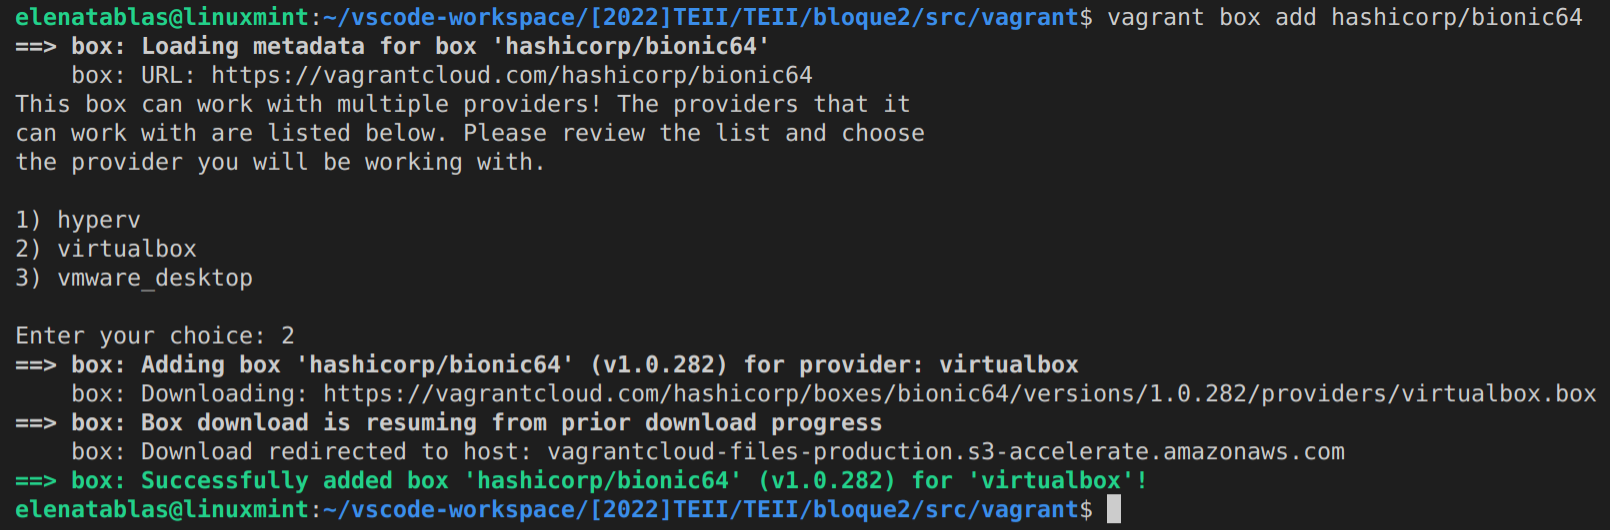
\includegraphics[width=\textwidth]{vagrant-box-add}
    \centering
    \caption{Instalación de \texttt{Ubuntu 18.04 LTS 64-bit box}.}
    \label{fig:vagrant-box-add}
 \end{figure}
\par \textbf{Segundo}, inicializo la \texttt{Box} que crea un archivo llamado \texttt{Vagrantfile} como 
se indica en la Figura \ref{fig:vagrant-box-init} y configuro mi proyecto para usarla como base.
 %%% IMAGEN VAGRANT BOX INIT %%%
\begin{figure}[H]
    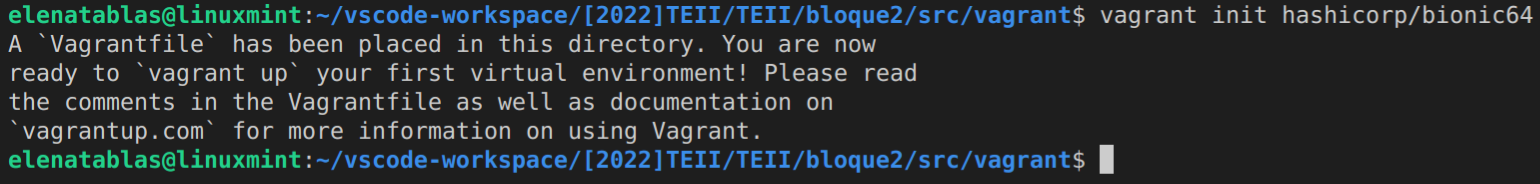
\includegraphics[width=\textwidth]{vagrant-box-init}
    \centering
    \caption{Inicialización de \texttt{Ubuntu 18.04 LTS 64-bit box}.}
    \label{fig:vagrant-box-init}
 \end{figure}
 \par Añado explícitamente dentro del fichero generado \texttt{Vagrantfile}, la versión y url de la \texttt{Box}.
 \begin{listing}
    Vagrant.configure("2") do |config|
        config.vm.box = "hashicorp/bionic64"
  +     config.vm.box_version = "1.0.282"
  +     config.vm.box_url = "https://vagrantcloud.com/hashicorp/bionic64"
    end
 \end{listing}

%%%%%%%%%%%%%%%%%%%%%%%%%%%%%%%%%%%%%%%%%%%%%%%%%%%%%%%%%%%%%%%%%%%%%%%%%%%%%%%%%%%%%%%%%%%%%%%%%%%%%%%%%%%%%%%%%%%%%%%%%%%%%%%%%%%%%%%%%%%%%%
\subsubsection{Configurar el servidor Apache con Vagrant en la VM creada (Usar el provider Shell de Vagrant para configurar e instalar el Apache automáticamente al crear la VM).}
\par \textbf{Primero}, creo un directorio llamado \texttt{html} en la carpeta donde está el fichero \texttt{Vagrantfile} 
y dentro del directorio el archivo \texttt{index.html}.
\begin{listing}[style=consola]
    $ mkdir html
    $ touch html/index.html
\end{listing}
\textbf{html/index.html}
\begin{listing}
    <!DOCTYPE html>
    <html>
        <body>
        <h1>Servidor web con Vagrant!!</h1>
        </body>
    </html>
 \end{listing}
 \par \textbf{Segundo}, escribo un archivo de provisión en el mismo directorio que \texttt{Vagrantfile}
 para intalar Apache al crear la máquina virtual.
 \textbf{bootstrap.sh}
 \begin{listing}
    #!/usr/bin/env bash

    apt-get update
    apt-get install -y apache2
    if ! [ -L /var/www ]; then
        rm -rf /var/www
        ln -fs /vagrant /var/www
    fi 
\end{listing}
\par \textbf{Tercero}, añado la línea \texttt{config.vm.provision :shell, path: "bootstrap.sh"}
 al fichero \textbf{Vagrantfile} antes del \texttt{end} para que lance el script anterior al inicio.
\begin{listing}
    Vagrant.configure("2") do |config|
        config.vm.box = "hashicorp/bionic64"
        config.vm.box_version = "1.0.282"
        config.vm.box_url = "https://vagrantcloud.com/hashicorp/bionic64"
  +     config.vm.provision :shell, path: "bootstrap.sh"
    end
 \end{listing}
 \par \textbf{Por último}, relanzo y configuro la VM con el shell \texttt{provisioner} que va a
 lanzar el script \texttt{bootstrap.sh}.
 \begin{listing}[style=consola]
    $ vagrant reload --provision
\end{listing}
\par Compruebo el funcionamiento del servidor, Figura \ref{fig:vagrant-ssh}.
  %%% IMAGEN VAGRANT SSH %%%
\begin{figure}[H]
    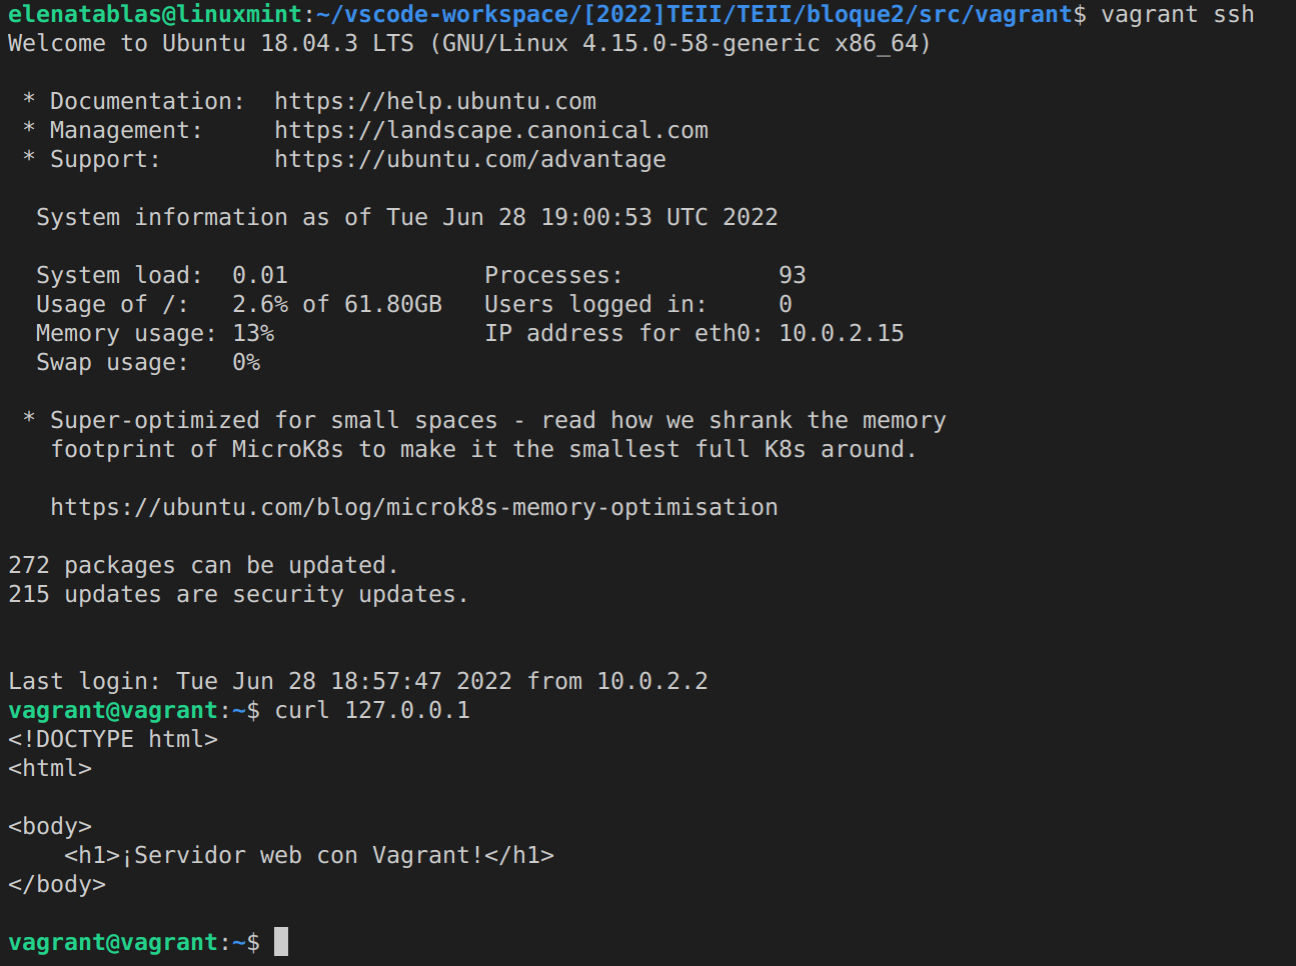
\includegraphics[width=\textwidth]{vagrant-ssh}
    \centering
    \caption{Compruebo el funcionamiento del servidor.}
    \label{fig:vagrant-ssh}
 \end{figure}
%%%%%%%%%%%%%%%%%%%%%%%%%%%%%%%%%%%%%%%%%%%%%%%%%%%%%%%%%%%%%%%%%%%%%%%%%%%%%%%%%%%%%%%%%%%%%%%%%%%%%%%%%%%%%%%%%%%%%%%%%%%%%%%%%%%%%%%%%%%%%%
\subsubsection{Redimensionar con Vagrant la máquina a 2GB de RAM y 2 CPUs.}
\par Para configurar la memoria y el número de CPUs de la máquina, tengo que ejecutar las 
siguientes líneas en el provider \textit{virtualbox} de Vagrant.
\begin{listing}
    Vagrant.configure("2") do |config|
        ...
  +     config.vm.provider "virtualbox" do |vb|
  +         # Customize the amount of memory on the VM:
  +         vb.memory = "2048"
  +         vb.cpus = 2
  +     end
    end
\end{listing}
\begin{listing}[style=consola]
    $ vagrant reload --provision
\end{listing}

%%%%%%%%%%%%%%%%%%%%%%%%%%%%%%%%%%%%%%%%%%%%%%%%%%%%%%%%%%%%%%%%%%%%%%%%%%%%%%%%%%%%%%%%%%%%%%%%%%%%%%%%%%%%%%%%%%%%%%%%%%%%%%%%%%%%%%%%%%%%%%
\subsubsection{Comprobar que podemos acceder desde la máquina virtual creada con Vagrant al servidor web de la otra máquina virtual creada con VboxManage y viceversa.}
\par Para que se pueda acceder desde otra máquina virtual, \textbf{primero} tengo que configurar el 
\texttt{PortForwarding} en el fichero vagrant. Hago que al hacer \texttt{localhost:8080} en
la máquina host, mapee al puerto \texttt{80} de la máquina virtual. Además, utilizo la misma 
red privada que permite \texttt{host-only} para poder conectarme con el host y el resto 
de maquinas virtuales que pertenecen a esa red.
\begin{listing}
    Vagrant.configure("2") do |config|
        config.vm.box = "hashicorp/bionic64"
        config.vm.box_version = "1.0.282"
        config.vm.box_url = "https://vagrantcloud.com/hashicorp/bionic64"
        config.vm.provision :shell, path: "bootstrap.sh"
  +     config.vm.network :forwarded_port, guest: 80, host: 8080
  +     # Create a private network, which allows host-only access to the machine
  +     # using a specific IP.
  +     config.vm.network "private_network", ip: "192.168.58.10"
    end
 \end{listing}
\begin{listing}[style=consola]
    $ vagrant reload --provision
\end{listing}
\par Compruebo que puedo acceder desde la máquina virtual creada con \texttt{Vagrant} al servidor web de la otra máquina virtual creada con \texttt{VboxManage}.
  %%% IMAGEN COMPROBACION VBOXMANAGE %%%
  \begin{figure}[H]
    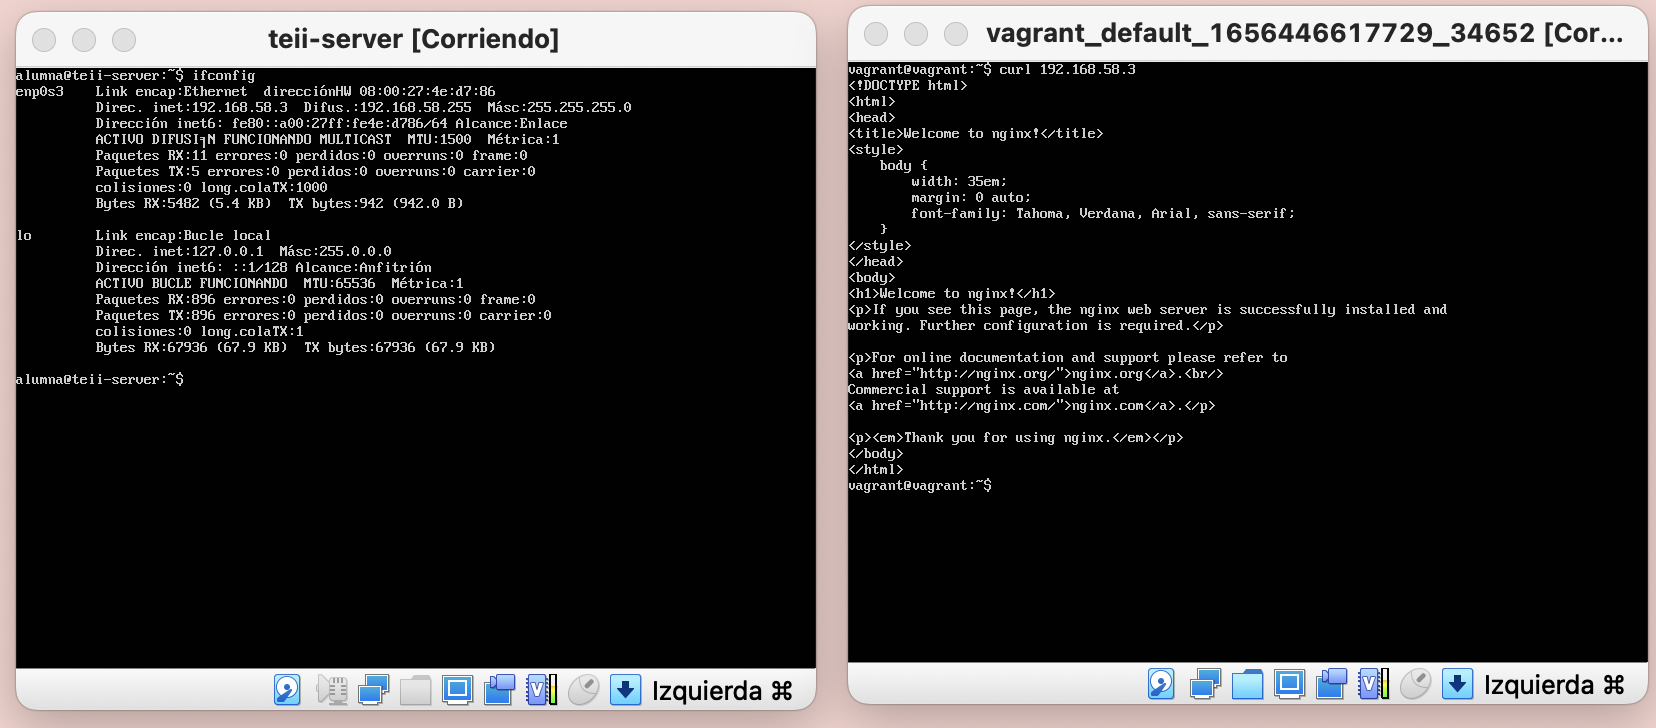
\includegraphics[width=\textwidth]{comprobacion-vboxmanage}
    \centering
    \caption{Compruebo el acceso al servidor creado por \texttt{VboxManage}.}
    \label{fig:comprobacion-vboxmanage}
 \end{figure}
\par Compruebo que puedo acceder desde la máquina virtual creada con \texttt{VboxManage} al servidor web de la otra máquina virtual creada con \texttt{Vagrant}.
  %%% IMAGEN COMPROBACION VAGRANT %%%
  \begin{figure}[H]
    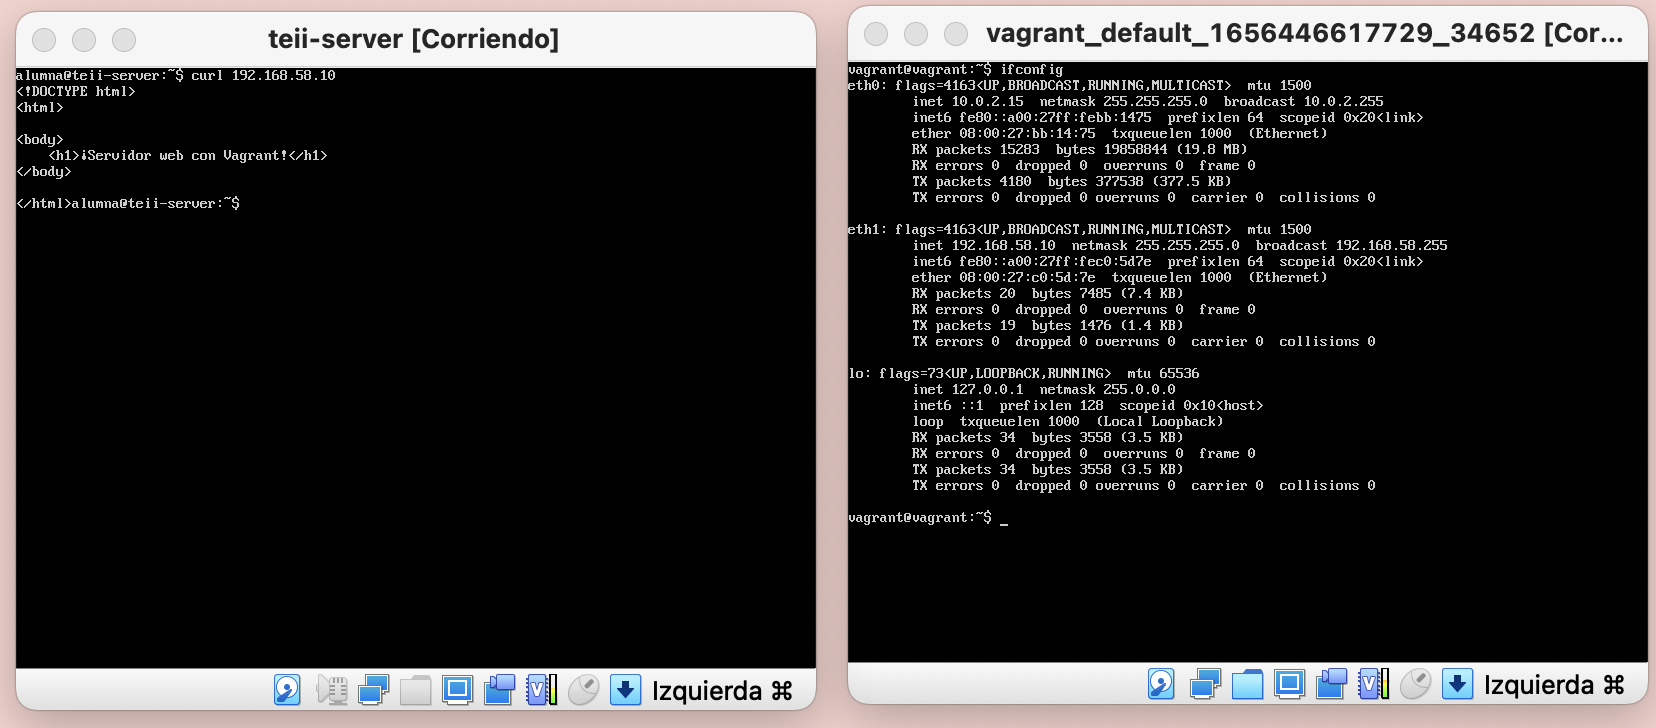
\includegraphics[width=\textwidth]{comprobacion-vagrant}
    \centering
    \caption{Compruebo el acceso al servidor creado por \texttt{Vagrant}.}
    \label{fig:comprobacion-vagrant}
 \end{figure}
%%%%%%%%%%%%%%%%%%%%%%%%%%%%%%%%%%%%%%%%%%%%%%%%%%%%%%%%%%%%%%%%%%%%%%%%%%%%%%%%%%%%%%%%%%%%%%%%%%%%%%%%%%%%%%%%%%%%%%%%%%%%%%%%%%%%%%%%%%%%%%
